\documentclass[11 pt]{beamer}

\usepackage[utf8]{inputenc}
\usepackage[T1]{fontenc}
\usepackage[french]{babel}

\usepackage{amsmath}
\usepackage{empheq}
\usepackage{tikz}
\usepackage{tikz-qtree}
\usepackage{listings}
\usepackage{graphicx}

\usepackage{xmpmulti}
\usepackage{animate}

\setbeamertemplate{itemize subitem}[square]
\setbeamertemplate{itemize subsubitem}[circle]

\title{Classification of points in a euclidean space}
\author{Luc Blassel, Romain Gautron}

\begin{document}
\maketitle

\begin{frame}{The problem}

\end{frame}

\begin{frame}[c]{A simple example}
  We have the following dataset in a $2d$ space:
  \begin{align*}
    X &=\{(1, 3),(1, 8), (2, 2), (2, 10), (3, 6), (4, 1), (5, 4), (6, 8), \\&(7, 4), (7, 7), (8, 2), (8, 5), (9, 9)\}\\
    &\\
    Y &= \{Blue,\ Blue,\ Blue,\ Blue,\ Blue,\ Blue,\ Red,\ Red,\ Red,\ Red,\ \\& Red,\ Red,\ Red \}
  \end{align*}
  We want to assign a color to the following point: $(4,8)$\
\end{frame}

\begin{frame}{What is being used today?}

\end{frame}

\begin{frame}{Knn}

\end{frame}

\begin{frame}{Knn}

\end{frame}

\begin{frame}{How to opitimze k-nn search}
  We use a data structure known as a k-d tree.
  \begin{itemize}
    \item
  \end{itemize}
\end{frame}

\begin{frame}

\end{frame}
\begin{frame}[shrink=22]{building the k-d tree}
  \begin{tikzpicture}[draw,circle,fill=none]
    \node[draw,fill=red] (0) at (0,0) {$(5,4)$};

    \node[draw,fill=green] (1) at (-4,-2) {$(3,6)$};
    \node[draw,fill=green] (2) at (4,-2 ) {$(7,7)$};

    \node[draw,fill=red] (3) at (-6,-4) {$(2,2)$};
    \node[draw,fill=red] (4) at (-2,-4) {$(2,10)$};
    \node[draw,fill=red] (5) at (2,-4 ) {$(8,2)$};
    \node[draw,fill=red] (6) at (6,-4 ) {$(9,9)$};

    \node[draw,fill=green] (7) at (-7,-6) {$(1,3)$};
    \node[draw,fill=green] (8) at (-5,-6) {$(4,1)$};
    \node[draw,fill=green] (9) at (-3,-6) {$(1,8)$};
    \node[draw,fill=green] (10) at (1,-6) {$(7,4)$};
    \node[draw,fill=green] (11) at (3,-6) {$(8,5)$};
    \node[draw,fill=green] (12) at (5,-6) {$(6,8)$};

    \draw (0)--(1);
    \draw (0)--(2);
    \draw (1)--(3);
    \draw (1)--(4);
    \draw (2)--(5);
    \draw (2)--(6);
    \draw (3)--(7);
    \draw (3)--(8);
    \draw (4)--(9);
    \draw (5)--(10);
    \draw (5)--(11);
    \draw (6)--(12);
  \end{tikzpicture}
\end{frame}

\begin{frame}{How do we partition the space?}
  \begin{figure}
    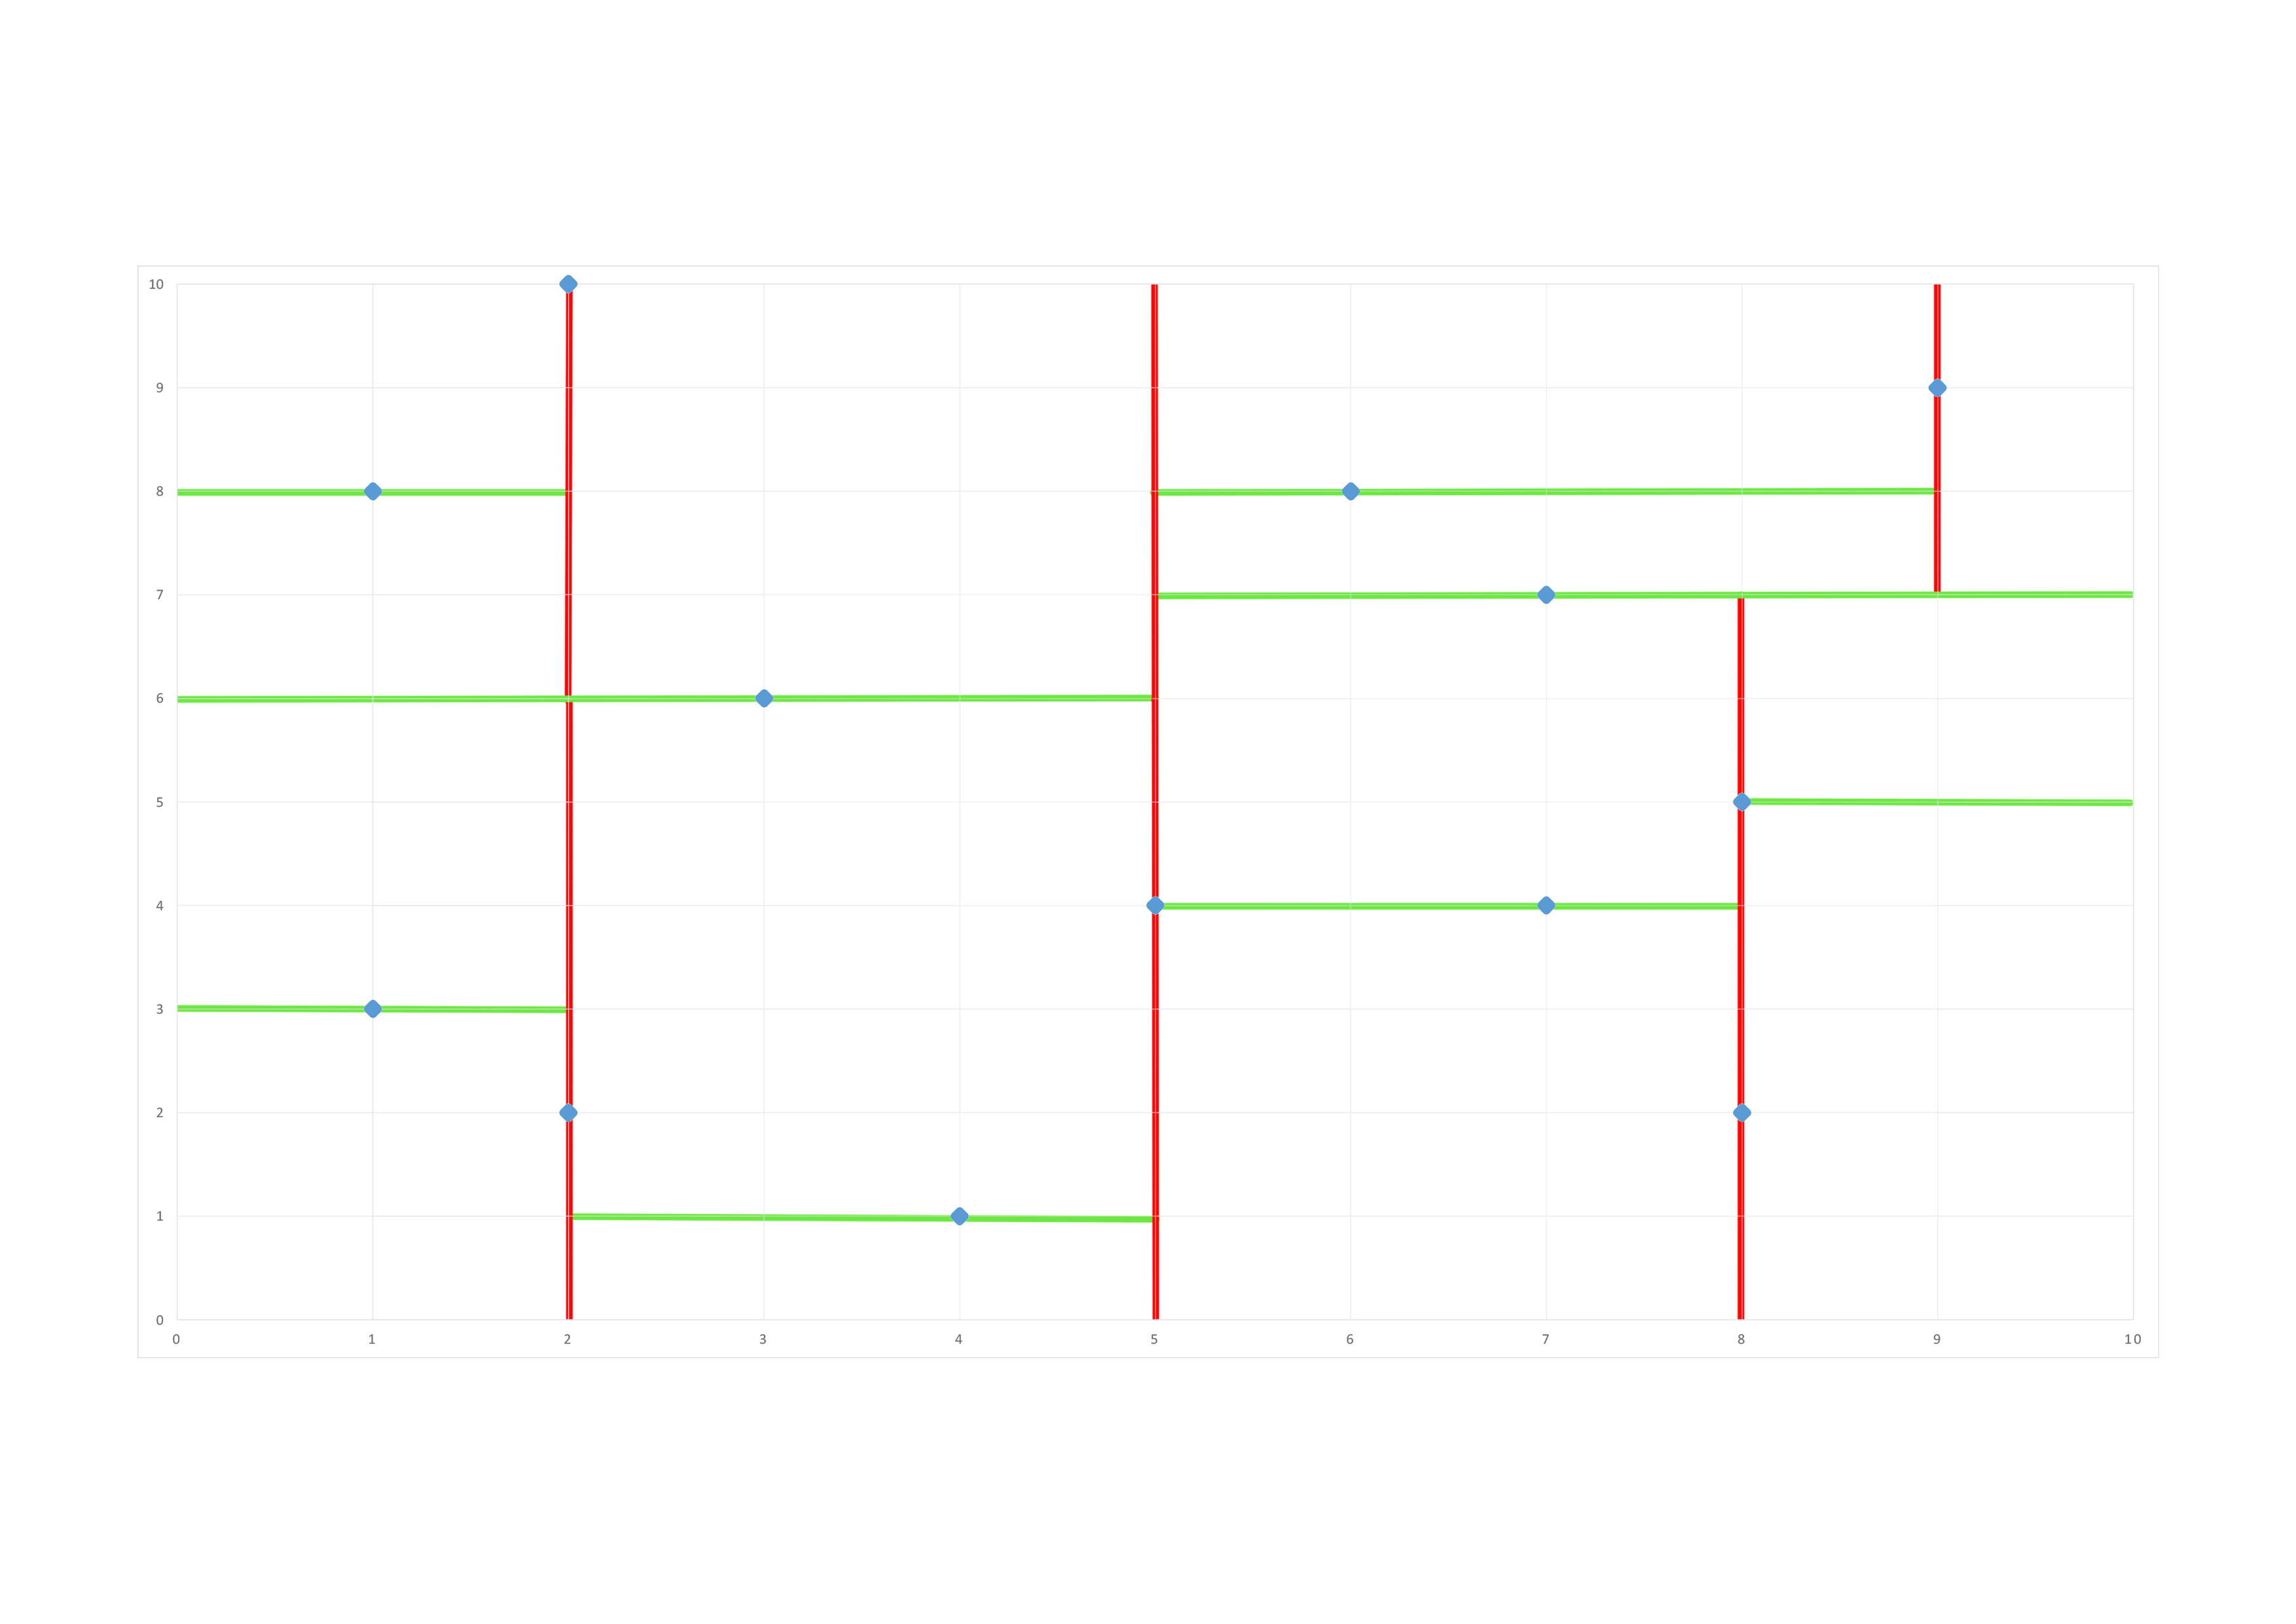
\includegraphics[width=\linewidth]{figures/splitFin.png}
    \caption{To animate}
  \end{figure}
\end{frame}

\begin{frame}{how do we find the k nearest neighbours?}
        \animategraphics[loop,controls,width=\linewidth]{10}{gif/cirle-}{0}{95}

\end{frame}

\begin{frame}{What is the time complexity?}
  For the tree creation (best case):
  \begin{align*}
    T(n) &= nlog(n)+2T\left(\frac{n}{2}\right)\\
         &= nlog(n)+2\left(\frac{n}{2}log\left(\frac{n}{2}\right)+2T\left(\frac{n}{4}\right)\right)\\
         &= nlog(n)+nlog\left(\frac{n}{2}\right)+4T\left(\frac{n}{4}\right)\\
         &= nlog(n)+nlog\left(\frac{n}{2}\right)+nlog\left(\frac{n}{4}\right)+\cdots+nlog\left(\frac{n}{2^{log(n)}}\right)\\
         &= n\sum^{log(n)}_{i=0}log\left(\frac{n}{2^i}\right)\\
         &= o\left(n\sum^{log(n)}_{i=0}log(n)\right)\\
         &= o(nlog^2(n))
  \end{align*}
\end{frame}

\begin{frame}{What is the time complexity?}
  For the tree creation (worst case):
  \begin{align*}
    T(n) &= n^2 +2T\left(\frac{n}{2}\right)\\
         &= n^2 +2\left(\left(\frac{n}{2}\right)^2+2T\left(\frac{n}{4}\right)\right)\\
         &= \sum^{log(n)}_{i=0}\frac{n^2}{2^i}\\
         &= n^3(2-2^{-log(n)})\\
         &= o(n^3)
  \end{align*}
\end{frame}

\begin{frame}{what is the time complexity}
  time complexity of our full program:
  \smallskip
  \begin{itemize}
  \item For the nearest neighbour search:
  \begin{itemize}
    \item best: $T(n)=o(log(n))$
    \item worst: $T(n)=o(n)$ \emph{$\equiv$ depth-first traversal}
  \end{itemize}
  \item For k-nearest neighbours of $p$ points:
  \begin{itemize}
    \item best:
    \begin{itemize}
      \item if $p>nlog(n) \Rightarrow T(n) = o(plog(n))$
      \item otherwise $T(n) = o(nlog^2(n))$
    \end{itemize}
    \item worst:
    \begin{itemize}
      \item if $p>n^2 \Rightarrow T(n)=o(pn)$ (very unlikely)
      \item otherwise $T(n)=o(n^3)$
    \end{itemize}
  \end{itemize}
\end{itemize}
\smallskip
Most of the complexity is due to tree creation.\\\smallskip
$k$-fold cross validation does not increase complexity unless the number of folds is very high.
\end{frame}

\begin{frame}{how does our algorithm perform in a real scenario}
  Using the Iris dataset:
  \begin{figure}
    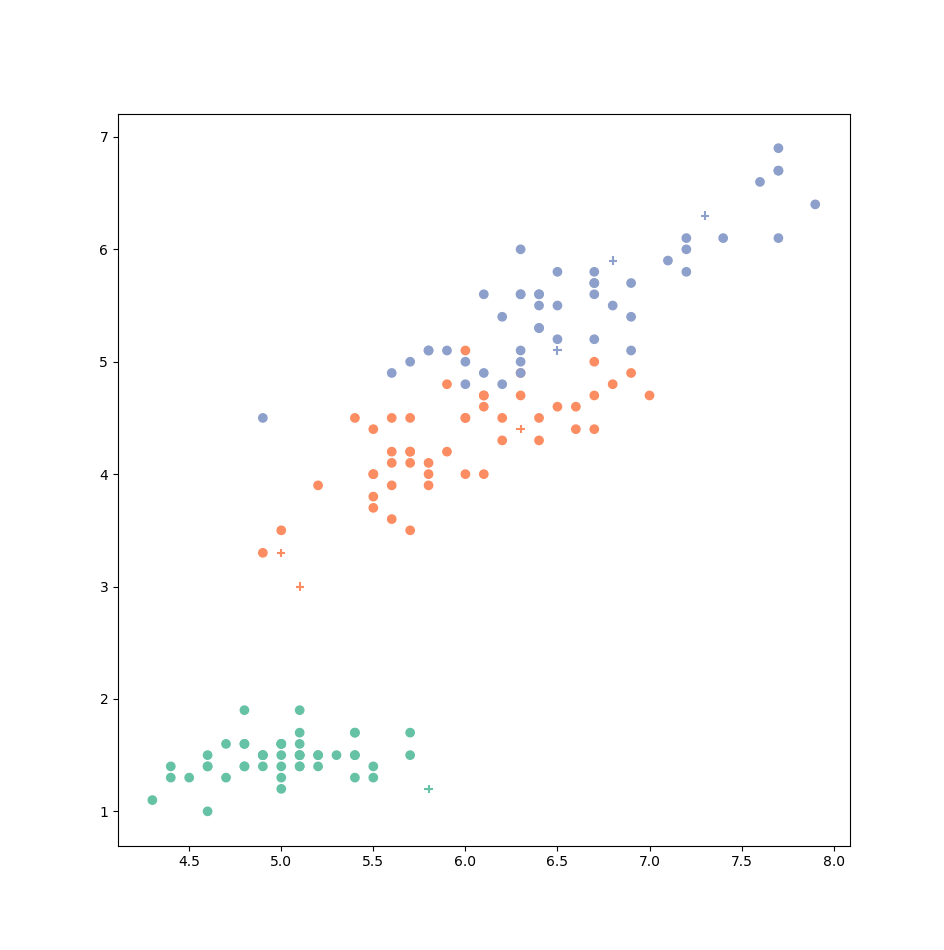
\includegraphics{figures/iris3.png}
    \caption{round points: known, crosses: classified points
  \end{figure}
\end{frame}

\end{document}
